\chapter{Survival analysis}

The \emph{survival analysis} is a regression model where the response is given by:
\begin{equation}
    T = \text{``Time until an event occurs''}\negthinspace,
\end{equation}
for example, the time until a patient dies, the time until a machine breaks down, etc.

\begin{example}
    A five-year medical study is conducted in which patients have been treated for cancer. The aim is to predict a patient survival time using features such as patient covariates, type of treatment, etc.

    However, some (hopefully many) patients may have survived until the end of the study. These patients have a survival time that is \emph{censored}. All we know is that it is at least five years, but we do not know its value. Other patients may have also dropped out of the study before its end. Survival analysis provides methods for this exact type of data.
\end{example}

There are also many other applications:
\begin{enumerate}
    \item Modelling churn, \ie, ``time until cancellation''\negthinspace.
    \item Modelling failure time of a product (reliability studies).
    \item The variable can also not be time.
    \item Time is naturally right-censored, but we can also have left-censoring, \eg, a pregnancy study where measurements start $250$ days after conception and $T$ is the time until the end of pregnancy.
    \item Another option is interval-censored data whether an event occurred during a specific period of time, like a week.
\end{enumerate}

\paragraph{Survival curve}

Let $T$ be:
\begin{equation}
    T = \text{``Time until an event occurs''}\negthinspace.
\end{equation}
There are different ways to describe $T$ probabilistically:
\begin{equation}
    \underset{\textsc{pdf}}{f(t)} = \P(T = t),\quad\qquad\underset{\textsc{cdf}}{F(t)} = \P(T \leq t),\quad\qquad\underset{\mathclap{\substack{\\\textsc{survival}\\\textsc{curve}}}}{S(t)} = \P(T > t) = 1 - F(t).
\end{equation}

\paragraph{Hazard function}

We define this function as:
\begin{equation}
    \begin{aligned}
        h(t) & = \lim_{\Delta t \to 0} \frac{\P(t < T \leq t + \Delta t \given T > t)}{\Delta t}              \\
             & = \lim_{\Delta t \to 0} \frac{\P(t < T \leq t + \Delta t) \cap \P(T > t)}{\P(T > t) \Delta t} \\
             & = \lim_{\Delta t \to 0} \frac{\P(t < T \leq t + \Delta t)}{S(t) \Delta t}                      \\
             & = \frac{1}{S(t)} \lim_{\Delta t \to 0} \frac{\P(t < T \leq t + \Delta t)}{\Delta t}            \\
             & = \frac{f(t)}{S(t)}\negthinspace.
    \end{aligned}
\end{equation}
The functions are all equivalent and can be used for modelling $T$:
\begin{equation}
    f(t) \longleftrightarrow F(t) \longleftrightarrow S(t) \longleftrightarrow h(t).
\end{equation}

\paragraph{Different models} There are different ways of modelling survival data:
\begin{enumerate}
    \item Non-parametric.
    \item Parametric (assuming a specific shape for the distribution of $T$).
    \item Semi-parametric.
\end{enumerate}

Now we set:
\begin{equation}
    \begin{aligned}
        T & = \text{``Survival time''}\negthinspace,  \\
        C & = \text{``Censoring time''}\negthinspace.
    \end{aligned}
\end{equation}
What we observe is:
\begin{equation}
    Y\negthinspace\colon \min(T\negthinspace, C) = \begin{cases}
        T & \text{if } T \leq C, \\
        C & \text{if } T > C.
    \end{cases}
\end{equation}
In addition, we observe:
\begin{equation}
    \delta = \begin{cases}
        1 & \text{if } T \leq C, \\
        0 & \text{if } T > C.
    \end{cases}
\end{equation}
that is a binary variable that indicates whether the event of interest occurred or not. For instance, if a person died or left the study before its end.

So, a dataset is given by $\set{\tuple{Y_i, \delta_i}}_{i=1}^n$.

\section{Kaplan-Meier estimator of survival curve}

\begin{figure}[ptb]
    \centering
    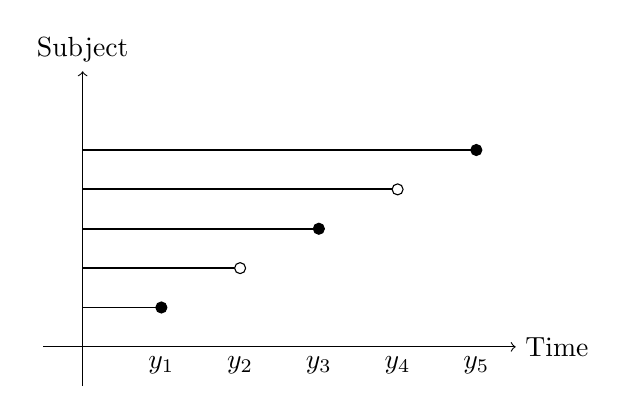
\begin{tikzpicture}[scale=1]
        \draw[->] (-0.5, 0) -- (5.5, 0) node[right] {Time};
        \draw[->] (0, -0.5) -- (0, 3.5) node[above] {Subject};

        \draw[line width=.7pt] (0, .5) -- (1, .5);
        \draw[line width=.7pt] (0, 1) -- (2, 1);
        \draw[line width=.7pt] (0, 1.5) -- (3, 1.5);
        \draw[line width=.7pt] (0, 2) -- (4, 2);
        \draw[line width=.7pt] (0, 2.5) -- (5, 2.5);

        \filldraw[fill=black, draw=black] (1, .5) circle (0.07);
        \filldraw[fill=white, draw=black] (2, 1) circle (0.07);
        \filldraw[fill=black, draw=black] (3, 1.5) circle (0.07);
        \filldraw[fill=white, draw=black] (4, 2) circle (0.07);
        \filldraw[fill=black, draw=black] (5, 2.5) circle (0.07);

        \node[below] at (1, 0) {$y_1$};
        \node[below] at (2, 0) {$y_2$};
        \node[below] at (3, 0) {$y_3$};
        \node[below] at (4, 0) {$y_4$};
        \node[below] at (5, 0) {$y_5$};
    \end{tikzpicture}
    \caption{Example of a dataset with $n=5$ subjects. The circles indicate whether the event of interest occurred (black) or not (white).}
\end{figure}

Suppose that we have the following dataset:
\begin{equation}
    \set{(y_1, 1), (y_2, 0), (y_3, 1), (y_4, 0), (y_5, 1)},
\end{equation}

We want to compute, for example:
\begin{equation}
    \hat{S}(y_3) = \hat{\P}(T > y_3).
\end{equation}

Some na\"ive options:
\begin{itemize}[beginpenalty=10000]
    \item Throw away missing observations:
          \begin{equation}
              \hat{S}(y_3) = \frac{1}{3},
          \end{equation}
          where we only consider the three subjects for which we are sure that the event of interest occurred (the black circles).
    \item Consider all observations:
          \begin{equation}
              \hat{S}(y_3) = \frac{2}{5},
          \end{equation}
          where we consider all the subjects, including those for which we are not sure that the event of interest occurred (the white circles), but we treat them as if they were black circles.
\end{itemize}
A better option would be to consider only time points at which the event of interest occurred. For example:
\begin{equation}
    \hat{S}(y_1) = \hat{\P}(T > y_1) = \frac{4}{5}.
\end{equation}
In this case we account also for patients $2$ and $4$. To compute $\hat{S}(y_3)$, we can use the following formula:
\begin{equation}
    \begin{aligned}
        \hat{S}(y_3) & = \hat{\P}(T > y_3)                                                                     \\
                     & = \P(T > y_3 \given T \leq y_1) \P(T \leq y_1) + \P(T > y_3 \given T > y_1) \P(T > y_1) \\
                     & = \hat{\P}(T > y_3 \given T > y_1) \hat{\P}(T > y_1)                                    \\
                     & = \frac{2}{3}\cdot \frac{4}{5} = \frac{8}{15}.
    \end{aligned}
\end{equation}
We used the fact that $\P(T > y_3 \given T \leq y_1) = 0$ since $y_3 > y_1$.
Obviously, we can also compute $\hat{S}(y_5)$:
\begin{equation}
    \hat{S}(y_5) = \hat{\P}(T > y_5) = 0,
\end{equation}
since there is no data point greater than $y_5$. The survival curve is, therefore, given by the step function showed in~\Cref{fig:survival-curve}.
\begin{figure}
    \centering
    \begin{tikzpicture}
        \draw[->] (-0.5, 0) -- (6, 0) node[right] {Time};
        \draw[->] (0, -0.5) -- (0, 2.5) node[above] {Survival probability};
        \draw[thick] (0, 2) -- (1, 2) -- (1, 1.5) -- (3, 1.5) -- (3, .9) -- (5, .9) -- (5, 0) -- (5.5, 0);

        \node[left] at (-0.5, 2) {$1$};
        \node[left] at (-0.5, 1.5) {$4/5$};
        \node[left] at (-0.5, 0.9) {$8/15$};

        \node[below] at (1, -0.5) {$y_1$};
        \node[below] at (3, -0.5) {$y_3$};
        \node[below] at (5, -0.5) {$y_5$};

        \draw[dashed] (1, 0) -- (1, 1.5);
        \draw[dashed] (3, 0) -- (3, .9);
    \end{tikzpicture}
    \caption{Kaplan-Meier estimator of the survival curve.}\label{fig:survival-curve}
\end{figure}

Usually, the time points are way more and the survival curve is smoother. Also, some observations reach the end of the study, so the survival curve does not go to zero on the right.

\paragraph{Non-parametric approach}

More formally, let a generic dataset be:
\begin{equation}
    d_1, \ldots, d_k\colon \text{ death times},
\end{equation}

Let $r_k$ be:
\begin{equation}
    r_k = \text{``Number of patients alive and in the study just before $d_k$''}\negthinspace.
\end{equation}
This is also called the \emph{risk set} at time $d_k$. Let $q_k$ be:
\begin{equation}
    q_k = \text{``Number of patients that died at time $d_k$''}\negthinspace.
\end{equation}
Then:
\begin{equation}
    \begin{aligned}
        S(d_k) & = \P(T > d_k \given T > d_{k-1}) \underbracket{\P(T > d_{k-1})}_{S(d_{k-1})} \\
               & = \prod_{j=1}^k \P(T > d_j \given T > d_{j-1})                               \\
    \end{aligned}
\end{equation}
is estimated using:
\begin{equation}
    \hat{\P}(T > d_j \given T > d_{j-1}) = \frac{r_j - q_j}{r_j},
\end{equation}
so that:
\begin{equation}
    \hat{S}(d_k) = \prod_{j=1}^k \frac{r_j - q_j}{r_j}, \quad k = 1, \ldots, K,
\end{equation}
and this is called the \emph{Kaplan-Meier estimator} of the survival curve (non-parametric estimator). For times $\tuple{d_k, d_{k+1}}$ we set $\hat{S}(t) = \hat{S}(d_k)$, so that the survival curve is a step function.

\begin{observation}
    This is similar to computing a histogram at the level of survival curves and considering missing data.
\end{observation}

\paragraph{Parametric approach}

We can assume that the distribution of $T$ has a certain parametric form. Then, $f(t)$, $F(t)$, $S(t)$ and $h(t)$ all depend on parameters.

Given $n$ observations of the form $\tuple{y_i, \delta_i}$, we compute the likelihood as:
\begin{equation}
    \begin{aligned}
        \L(\thetavec) & = \prod_{i=1}^n f(y_i)^{\delta_i} S(y_i)^{1 - \delta_i}              \\
           & = \prod_{i=1}^n \left(\frac{f(y_i)}{S(y_i)}\right)^{\delta_i} S(y_i) \\
           & = \prod_{i=1}^n h(y_i)^{\delta_i} S(y_i).
    \end{aligned}
\end{equation}
If we assume that $T$ is exponentially distributed, then:
\begin{equation}
    \begin{aligned}
        f(t) & = \lambda e^{-\lambda t}\negthinspace,    \\
        F(t) & = 1 - e^{-\lambda t}\negthinspace,        \\
        S(t) & = 1 - F(t) = e^{-\lambda t}\negthinspace, \\
        h(t) & = \frac{f(t)}{S(t)} = \lambda.
    \end{aligned}
\end{equation}
Then, $\lambda$ is estimated via maximum likelihood:
\begin{equation}
    \L(\lambda) = \prod_{i=1}^n \lambda^{\delta_i} e^{-\lambda y_i} \implies \hat{\lambda} = \argmax_{\lambda} \L
\end{equation}
and the survival curve is estimated as:
\begin{equation}
    \hat{S}(t) = e^{-\hat{\lambda} t}\negthinspace.
\end{equation}

\paragraph{Regression approaches}

Here we want to predict $T$ from a number of covariates $X_1, \ldots, X_p$. {Non-parametric} approaches can be used in this case as well, but they require some stratification of the observations into groups, which is not really feasible for a large number of predictors. With one predictor, \eg $X = \text{``Gender''}\negthinspace$, one could split data into males and females and compute a Kaplan-Meier curve for each group. After having computed the curves, we can conduct a \emph{log-rank test} to determine if differences between the two are statistically significant.

It is easier to account for covariates under a parametric approach. For example, is one assume an exponential distribution, we could make this assumption conditional on $\xvec$, like in \acsp{glm}:
\begin{equation}
    T \given \Xvec = \xvec \sim \exponential(\lambda(\xvec)),
\end{equation}
with $\log(\lambda(\xvec)) = \beta_0 + \betavec^\t\xvec$. In particular:
\begin{equation}
    \log(\lambda(\xvec_i)) = \log(h(t \given \xvec_i)) = \beta_0 + \betavec^\t\xvec_i, \quad i = 1, \ldots, n.
\end{equation}
The likelihood now depends on $\beta_0$ and $\betavec$:
\begin{equation}
    \hat{\lambda}(\xvec) = \exp(\hat{\beta}_0 + \hat{\betavec}^\t\xvec)
\end{equation}
and we have a survival curve for each realization $\xvec$ of the covariates:
\begin{equation}
    \hat{S}(t \given \xvec) = \exp(-\hat{\lambda}(\xvec) t).
\end{equation}
The curve is, therefore, typically plotted by fixing all covariates to a level (for example, mean, mode, etc.) and changing one variable only ($x_j$) to see how the curve changes with respect to it.

\begin{note}
    The exponential may be too restrictive in many applications. Weibull distribution (with two parameters) is quite common in engineering (reliability modelling).
\end{note}